\section{Q3} 

\subsection{Introduction} \label{sec:Introduction}

Freight elevators are essential systems in industrial and commercial environments, providing reliable 
vertical transportation of materials between different levels of a facility. In this laboratory exercise, 
the goal is to design and implement an electromagnetic control system to automate the operation of a freight 
elevator, using a three-phase motor managed by contactors and safety devices.

The proposed system must fulfill a specific set of operational requirements, including conditional 
upward and downward movement, timed delays, and immediate interruption in case of an emergency stop. 
Additionally, the system incorporates status indicators, such as lamps and sirens, to enhance operational 
safety and monitoring.

This report details the development of the control strategy through a Grafcet diagram, capturing the 
sequence of states and transitions governing the elevator’s operation. From this, the assembly diagram 
is created, illustrating the interconnections between all components and their terminal numbering. The 
electrical power and command circuits are subsequently derived and implemented in Fluidsim 3.6, enabling 
simulation and validation of the system’s compliance with the defined specifications.

The exercise reinforces critical concepts in industrial control, including the integration of safety 
mechanisms, timed operations, and the coordination of electrical and pneumatic components within an 
automated process.

\subsection{Grafcet Representation} \label{sec:Grafcet_Representation}

\begin{figure}[H]
    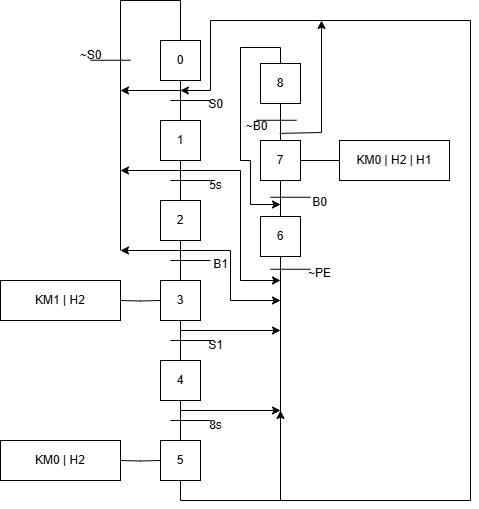
\includegraphics[width=16cm]{Images/Q3/grafset.png}
    \centering
    \caption{Grafset for the freight elevator}
    \label{fig:grafset}
\end{figure}

\subsection{Electrical Power Circuit Diagram} \label{sec:Electrical_Power_Circuit_Diagram}

\begin{comment}
    NOTA: ACRESCENTAR A FIGURA
    \begin{figure}[H]
    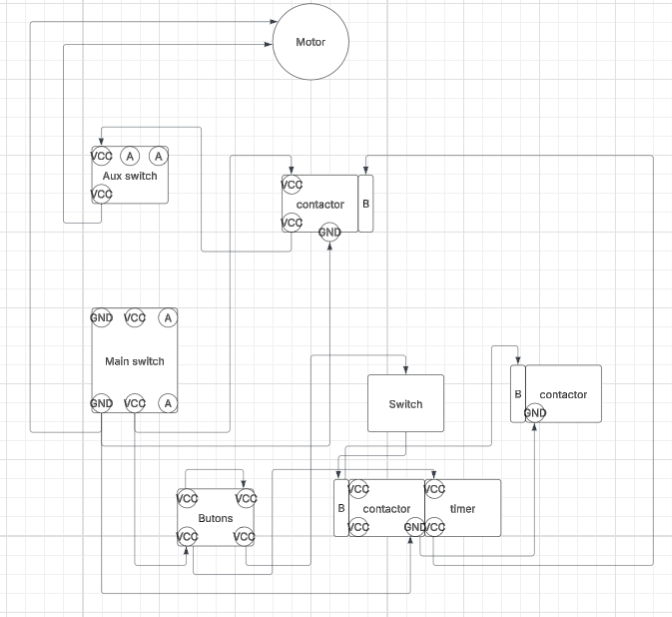
\includegraphics[width=16cm]{Images/Q2/eletrical_circuit.png}
    \centering
    \caption{Decided schematic for the door control}
    \label{fig:eletrical_circuit}
\end{figure}
\end{comment}

\subsection{Electrical Command Circuit Diagram} \label{sec:Electrical_Command_Circuit_Diagram}

\begin{comment}
    NOTA: ACRESCENTAR A FIGURA
    \begin{figure}[H]
    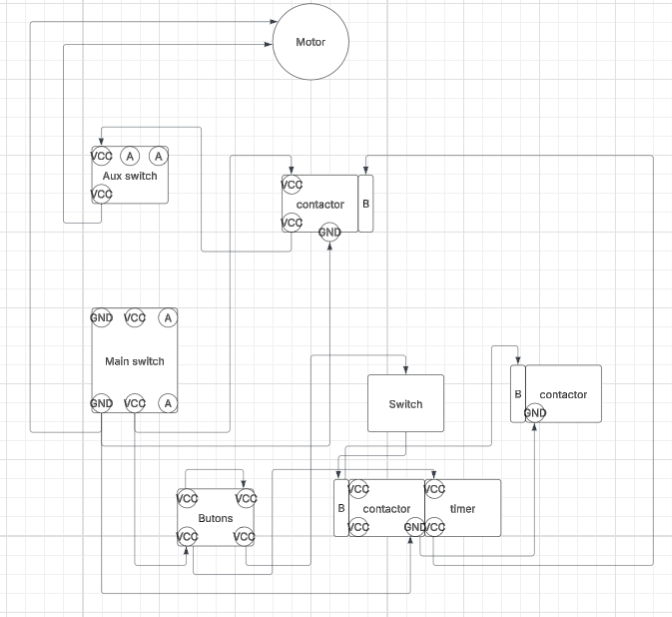
\includegraphics[width=16cm]{Images/Q2/eletrical_circuit.png}
    \centering
    \caption{Decided schematic for the door control}
    \label{fig:eletrical_circuit}
\end{figure}
\end{comment}

\subsection{Simulation and Validation} \label{sec:Simulation_and_Validation}

\begin{figure}[H]
    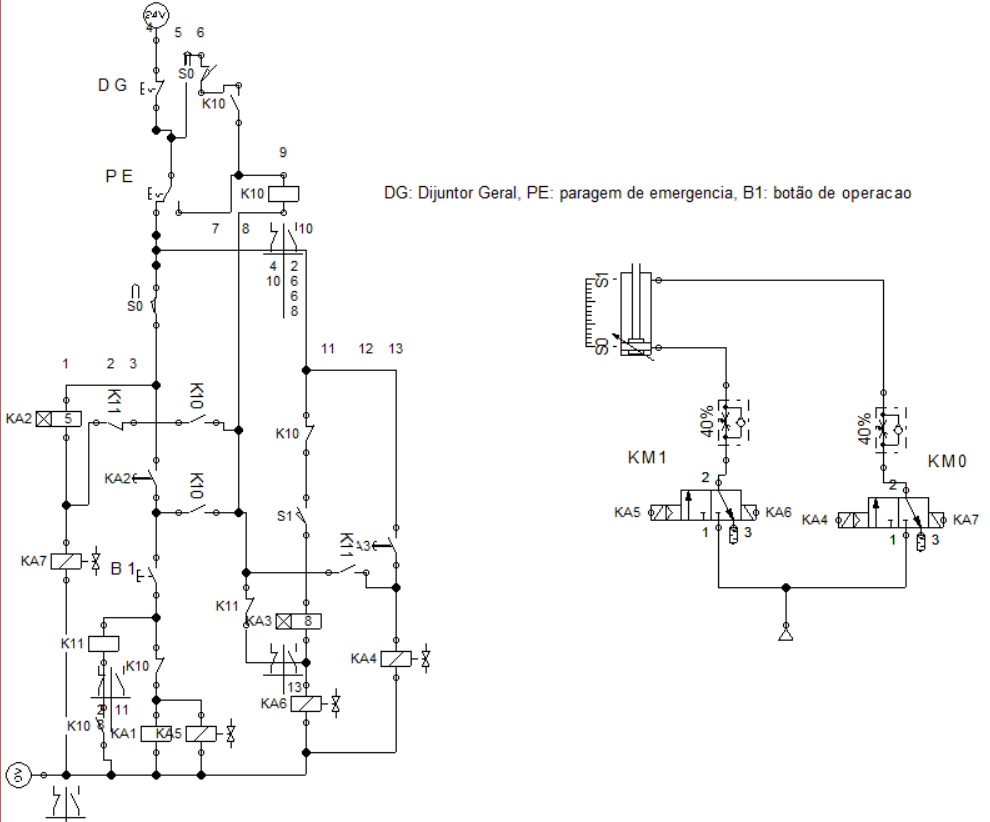
\includegraphics[width=16cm]{Images/Q3/fluidsim.png}
    \centering
    \caption{Fluidsim for the cargo elevator}
    \label{fig:fluidsim}
\end{figure}

\subsection{Assembly Diagram} \label{sec:Assembly_Diagram}

\begin{comment}
    NOTA: ACRESCENTAR A FIGURA
    \begin{figure}[H]
    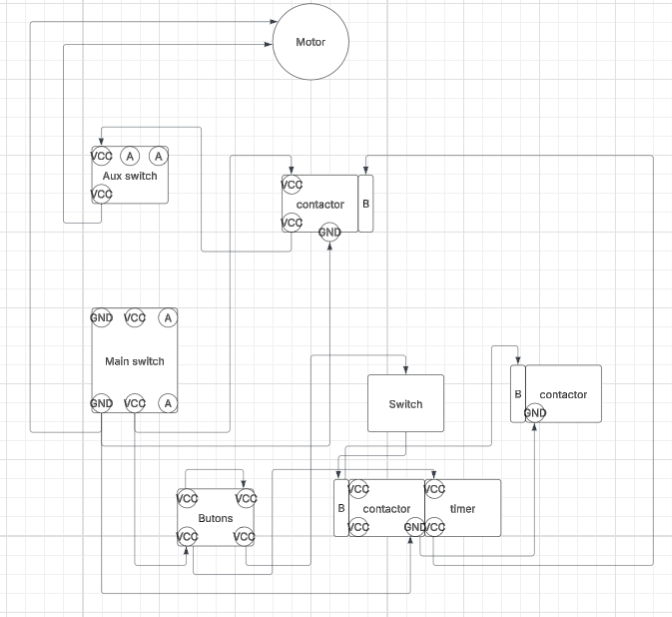
\includegraphics[width=16cm]{Images/Q2/eletrical_circuit.png}
    \centering
    \caption{Decided schematic for the door control}
    \label{fig:eletrical_circuit}
\end{figure}
\end{comment}

\subsection{Conclusion}

This report details the complete development of an electropneumatic control system, from schematic 
design to simulation validation. By integrating various automation components and methodologies, 
the system achieves a robust and efficient control mechanism. The findings highlight the importance 
of precise component selection and control logic design in achieving a functional and reliable 
automated process.